\begin{ex}%[2H5C3-3]
	Trong không gian với hệ tọa độ $Oxyz$, cho các điểm $A(1;0;0)$, $B(3;2;0)$, $C(-1;2;4)$. Gọi $M$ là điểm thay đổi sao cho đường thẳng $MA$, $MB$, $MC$ hợp với mặt phẳng $(ABC)$ các góc bằng nhau; $N$ là điểm thay đổi nằm trên mặt cầu $(S)\colon (x-3)^2+(y-2)^2+(z-3)^2 = \dfrac{1}{2}$. Tính giá trị nhỏ nhất của độ dài đoạn $MN$.
	\choice{$\dfrac{3\sqrt{2}}{2}$}{$\sqrt{2}$}{$\dfrac{\sqrt{2}}{2}$}{$\sqrt{5}$}
	\loigiai{	
		\begin{center}
				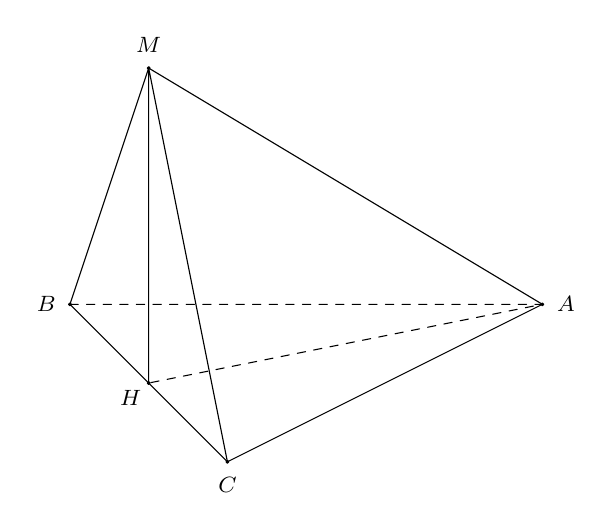
\begin{tikzpicture}[scale=1, font=\footnotesize, line join=round, line cap=round,>=stealth]
				\coordinate (A) at (6,0);
				\coordinate (B) at (0,0);
				\coordinate (C) at (2,-2);
				\coordinate (H) at (1,-1);
				\coordinate (M) at (1,3);
			\draw (B)--(M)--(A)--(C)--(B)--cycle;	
			\draw (H)--(M)--(C);			
				\draw[dashed](B)--(A)--(H);
				\foreach \p/\g in {A/0,B/180,C/-90,M/90,H/-140} \draw[fill] (\p) circle(.5pt) node [shift={(\g:.3)}] {$\p$};
			\end{tikzpicture}
		\end{center}
Ta có $\overrightarrow{AB} = (2; 2; 0)$, $\overrightarrow{AC} = (-2; 2; 4) \Rightarrow \overrightarrow{AB} \cdot \overrightarrow{AC} = 0 \Rightarrow \triangle ABC$ suy ra $\triangle ABC$ vuông tại $A$.\\
Gọi $H$ là hình chiếu vuông góc của điểm $M$ trên mặt phẳng $(ABC)$. Ta có\\
$(MA, (ABC)) = (MA, HA) = \widehat{MAH}$.\\
$(MB, (ABC)) = (MB, HB) = \widehat{MBH}$.\\
$(MC, (ABC)) = (MC, HC) = \widehat{MCH}$.\\
Theo giả thiết $\widehat{MAH} = \widehat{MBH} = \widehat{MCH} \Rightarrow \triangle MAH = \triangle MBH = \triangle MCH$ (g.c.g).\\
Do đó $HA = HB = HC$ nên $H$ là tâm đường tròn ngoại tiếp $\triangle ABC$.\\
Suy ra $H$ là trung điểm của $BC \Rightarrow H(1; 2; 2)$.\\
Ta có $\left[\overrightarrow{AB}, \overrightarrow{AC}\right] = (8; -8; 8)$, chọn vec-tơ chỉ phương của đường thẳng $MH$ là $\overrightarrow{u}_{MH} = (1; -1; 1)$.\\
Phương trình đường thẳng $MH$ có dạng:\\
$$\heva{&x = 1 + t \\&	y = 2 - t \\&	z = 2 + t}\quad (t \in \mathbb{R}).$$
Mặt cầu $(S)$ có tâm $I(3; 2; 3)$ và bán kính $R = \dfrac{\sqrt{2}}{2}$.
\begin{center}
	\begin{tikzpicture}[scale=0.9, font=\footnotesize, line join=round, line cap=round,>=stealth]
		\coordinate (I) at (0,0);
		\coordinate (B) at (2,0);
	\coordinate (N) at ($(I)!1!-100:(B)$);
	\draw (I)circle (2);
	\coordinate (M) at ($(I)!1.5!(N)$);
		\coordinate (c) at ($(M)!1!-90:(I)$);
		\coordinate (d) at ($(c)!1.7!(M)$);
		\draw (c)--(d) (I)--(M);	
		\foreach \p/\g in {I/90,M/-95,N/-50} \draw[fill] (\p) circle(.5pt) node [shift={(\g:.3)}] {$\p$};
	\end{tikzpicture}
\end{center}
Gọi $K(1+t; 2-t; 2+t)$ là hình chiếu vuông góc của điểm $I$ trên đường thẳng $MH$.\\
Ta có $\overrightarrow{IK} = (t-2; -t-1; t-1)$, $\overrightarrow{u}_{MH} = (1; -1; 1)$\\
Do $IK \perp MH$ nên $\overrightarrow{IK} \cdot \overrightarrow{u}_{MH} = 0$, ta được $t = 1$. Khi đó $K(2; 1; 3)$ và $IK = \sqrt{2}$\\
Do $IK > R$ nên đường thẳng $MH$ không cắt mặt cầu.\\
Ta có $MN \geq \mathrm{d}(I, MH) - IN = IK - IN = \dfrac{\sqrt{2}}{2}.$
}
\end{ex}
\begin{ex}%[2H5C3-3]
	Trong không gian với hệ tọa độ $Oxyz$, cho điểm $A(1;2;-3)$ và mặt phẳng $(P)\colon 2x+2y-z+9=0$. Đường thẳng $d$ đi qua $A$ và có vec-tơ chỉ phương $\vec{u}=(3;4;-4)$ cắt $(P)$ tại điểm $B$. Điểm $M$ thay đổi trong $(P)$ sao cho $M$ luôn nhìn đoạn $AB$ dưới góc $90^\circ$. Khi độ dài $MB$ lớn nhất, đường thẳng $MB$ đi qua điểm nào trong các điểm sau?
	\choice{$J(-3;2;7)$}{$K(3;0;15)$}{$H(-2;-1;3)$}{$I(-1;-2;3)$}
	\loigiai{
		\begin{center}
			\begin{tikzpicture}[scale=1,>=stealth, font=\scriptsize, line join=round, line cap=round,declare function={R=2;goc=-30;k=0.3;gocbu=180-goc;}]
			\pgfmathsetmacro\R{R}
			\pgfmathsetmacro\r{R*cos(goc)}
			\pgfmathsetmacro\a{.2*R}
			\pgfmathsetmacro\b{.2*\r}
			\pgfmathsetmacro\m{\r *cos(-50)}
			\pgfmathsetmacro\n{\b *sin(-50)}
			\path
			(0,0) coordinate (E)
			(-4,-1.5) coordinate (M')
			(2.5,-1.5) coordinate (N)
			(R,0)coordinate (A1)
			(-R,0)coordinate (A')
			(E)+(goc:R)coordinate (C)
			(E)+(-180-goc:R)coordinate (C')
			(barycentric cs:C'=1,C=1)coordinate(F)
			($(M')!2!(F)$)coordinate(P)
			($(N)!2!(F)$)coordinate(Q)
			($(Q)+(0.5,0)$)coordinate(K)
			($(P)+(-2.1,0)$)coordinate(T)
			;
			\path (F);
			\pgfgetlastxy{\xf}{\yf}
			\path
			($(F)+(\m,\n)$) coordinate (B)
			($(B)!2!(F)$)coordinate(M)
			($(B)!2!(E)$)coordinate(A)
			($(B)!2.5!(E)$)coordinate(d)
			;
			\draw (E)circle(R);
			\draw[dashed] (A1) arc (0:180:\R cm and \a cm);
			\draw[dashed] (C) arc (0:180:\r cm and \b cm);
			\draw[dashed] (M)--(B)--(A);
			\draw[dashed] (E)--(F);
			\draw (K)--(Q)--(M')--(N)--(P)--(T);
			\draw[dashed] (K)--(T);	
			\draw (A)--(d)node[above right]{$d$};
			\draw (A1) arc (0:-180:\R cm and \a cm);
			\draw (C) arc (0:-180:\r cm and \b cm);
			%			\draw (H)--(M)--(H') (M)--(X);
			\foreach \p/\g in{E/15,F/-100,B/45,M/-90,A/20}
			\shade[shading=ball](\p)circle(.03)node[shift={(\g:.25)},scale=1]{$\p$};
		\end{tikzpicture}
		\end{center}
Đường thẳng $d$ đi qua $A$ và có vec-tơ chỉ phương $\overrightarrow{u} = (3; 4; -4)$ có phương trình là 
$$\dfrac{x-1}{3} = \dfrac{y-2}{4} = \dfrac{z+3}{-4}.$$ 
Tính được giao điểm của $d$ và $(P)$ là $B = (-2; -2; 1)$.\\ Do $M$ luôn nhìn đoạn $AB$ dưới góc $90^\circ$ nên $M$ nằm trên mặt cầu $(S)$ đường kính $AB$.\\
Gọi $E$ là trung điểm của $AB \Rightarrow E = \left(-\dfrac{1}{2}; 0; -1\right) \Rightarrow AE^2 = \dfrac{41}{4}$.\\
$\Rightarrow (S)\colon x^2 + y^2 + z^2 + x + 2z - 9 = 0$.\\
Lại do $M \in (P)$ nên $M$ nằm trên đường tròn giao tuyến của mặt phẳng $(P)$ và mặt cầu $(S)$, gọi là đường tròn $(C)$.\\
 Mặt khác $B$ là điểm cố định trên đường tròn $(C)$ nên độ dài $MB$ lớn nhất khi $MB$ là đường kính của đường tròn $(C)$.\\
 Gọi $F$ là tâm của $(C) \Rightarrow F$ là hình chiếu vuông góc của $E$ trên $(P)$.\\
Đường thẳng $EF$ nhận vec-tơ pháp tuyến $\overrightarrow{n} = (2; 2; -1)$ của $(P)$ làm vec-tơ pháp tuyến. Suy ra $EF$ có phương trình
$$ \dfrac{x + \frac{1}{2}}{2} = \dfrac{y}{2} = \dfrac{z + 1}{-1}.$$
Từ đó ta tính được $F = \left( -\dfrac{5}{2}; -2; 0 \right)$ (là giao điểm của $(P)$ và $EF$).\\
 Vì $MB$ là đường kính của $(C)$ nên $M = (-3; -2; -1) \Rightarrow \overrightarrow{MB} = (1; 0; 2)$ là vec-tơ chỉ phương của đường thẳng $MB \Rightarrow$ phương trình đường thẳng $MB$ là 
$$\heva{&x=-2+t\\&y=-2\\&z=1+2t} \quad (t \in \mathbb{R}).$$
 Trong các điểm đã cho ở các phương án chỉ có điểm $I (-1; -2; 3)$  thuộc đường thẳng $MB$.	
}
\end{ex}
\begin{ex}%[2H5C2-6]
	Trong không gian với hệ tọa độ $Oxyz$, cho mặt cầu $(S)$ có tâm $I(1;2;3)$ và có bán kính $r=2$. Xét đường thẳng $d \colon \heva{&x=1+t \\&	y=-mt \\&	z=(m-1)t }\quad
		(t \in \mathbb{R})$, $ m$ là tham số  thực. \\
		Giả sử $(P), (Q)$ là mặt phẳng chứa $d$ và tiếp xúc với $(S)$ lần lượt tại $M, N$. Khi đó đoạn $MN$ ngắn nhất hãy tính khoảng cách từ điểm $B(1;0;4)$ đến đường thẳng $d$.
	\choice{$\sqrt{5}$}{$\dfrac{5\sqrt{3}}{3}$}{$\dfrac{4\sqrt{237}}{21}$}{\True$\dfrac{4\sqrt{273}}{21}$}
	\loigiai{
		\begin{center}
			\begin{tikzpicture}[scale=0.9, font=\footnotesize, line join=round, line cap=round,>=stealth]
				\coordinate (I) at (0,0);
				\coordinate (N) at (2,0);
			\coordinate (M) at($(I)!1!120:(N)$);				
				\coordinate (c) at ($(M)!1!90:(I)$);
				\coordinate (d) at ($(N)!1!-90:(I)$);
			\coordinate (H) at (intersection of M--c and N--d);
				\draw (I)circle (2);
		\draw (I)--(M)--(H)--(N)--(I)--cycle;
		\draw (H)--(I);	
		\draw pic[draw,angle radius=2mm] {right angle = I--M--H};
		\draw pic[draw,angle radius=2mm] {right angle = H--N--I};
		\foreach \p/\g in {I/-90,M/120,N/0,H/70} \draw[fill] (\p) circle(.5pt) node [shift={(\g:.3)}] {$\p$};
			\end{tikzpicture}
		\end{center}
Mặt phẳng thiết diện đi qua tâm $I, M, N$ cắt đường thẳng $d$ tại $H$.\\
 Suy ra $IH \perp d$, $\mathrm{d}(I, d) = IH$.\\
Ta có 
$$MN = 2MK = 2 \cdot \dfrac{MH \cdot MI}{IH} = 2 \cdot \dfrac{\sqrt{IH^2 - r^2} \cdot r}{IH} = \dfrac{4 \sqrt{IH^2 - 4}}{IH}.$$ 
Đặt $x = IH > 2$, ta có hàm số $ f(x)= \dfrac{4 \sqrt{x^2 - 4}}{x}$. \\
Ta có $f'(x) = \dfrac{4}{x^2 \sqrt{x^2 - 4}} > 0, \forall x > 2$, suy ra hàm số đồng biến trên $(2; +\infty)$.\\
Do đó $MN_{\text{min}} \Leftrightarrow IH_{\text{min}}$.\\
 Ta có $\overrightarrow{u}_d = (1; -m; m-1)$, $A(1; 0; 0) \in d$, suy ra
 $$\mathrm{d}(I, d) = \dfrac{\left| \overrightarrow{u}_d, \overrightarrow{IA} \right|}{|\overrightarrow{u}_d|}=\dfrac{\sqrt{25m^2 - 20m + 17}}{\sqrt{2m^2 - 2m + 2}}.$$
Xét hàm số $f(m) = \dfrac{25m^2 - 20m + 17}{2m^2 - 2m + 2}$ có bảng biến thiên là
	\begin{center}
	
\begin{tikzpicture}[>=stealth]
		\tkzTabInit[nocadre=false,lgt=1.5,espcl=2,deltacl=0.5]
		{$m$/.7 ,$f'(m)$/.7,$f(m)$/2}
		{$-\infty$ , $\frac{1}{5}$ , $3$ , $+\infty$}
		\tkzTabLine{ , - , $0$ , + , $0$ , - , }
		\tkzTabVar{+/$\frac{25}{2}$ , -/$\frac{25}{3}$, +/$13$ ,  -/$\frac{25}{2}$}
	\end{tikzpicture}	
\end{center}

Suy ra $IH_{\text{min}}$ khi $m = \dfrac{1}{5}$. Đường thẳng $d$ có phương trình là\\
$$\heva{&x = 1 + t \\ &y = -\dfrac{1}{5}t \\ &z = -\dfrac{4}{5}t} \quad (t \in \mathbb{R}).$$
Khoảng cách $\mathrm{d}(B, d) = \dfrac{\left| \overrightarrow{AB}, \overrightarrow{u}_d \right|}{|\overrightarrow{u}_d|} = \dfrac{\sqrt{416}}{\sqrt{42}} = \dfrac{4 \sqrt{273}}{21}$.

}
\end{ex}
\begin{ex}%[2H5C2-5]
	Trong không gian $Oxyz$, cho mặt phẳng $(P)\colon 2x+2y-z+9=0$ và điểm $A(1;2;-3)$. Đường thẳng $d$ đi qua $A$ và có véc-tơ  chỉ phương $\vec{u} = (3;4;-4)$ cắt $(P)$ tại $B$. Điểm $M$ thay đổi trên $(P)$ sao cho $M$ luôn nhìn đoạn $AB$ dưới một góc $90^\circ$. Độ dài đoạn $MB$ lớn nhất bằng
	\choice{$\dfrac{36}{\sqrt{5}}$}{$\sqrt{41}$}{$6$}{\True$\sqrt{5}$}
	\loigiai{
Phương trình đường thẳng $d\colon \heva{&x = 1 + 3t\\&y = 2 + 4t\\&z = -3 - 4t}$ nên tọa độ điểm $B$ thỏa mãn hệ phương trình \\
$\heva{&x = 1 + 3t\\&y = 2 + 4t\\&z = -3 - 4t\\&2x + 2y - z + 9 = 0} \Rightarrow 2(1 + 3t) + 2(2 + 4t) - (-3 - 4t) + 9 = 0 \Leftrightarrow t = -1 \Rightarrow B(-2; -2; 1)$.\\
Do $M$ nhìn đoạn $AB$ dưới một góc $90^\circ$ nên $M$ thuộc mặt cầu $(S)$ có đường kính $AB = \sqrt{41}$. Lại do $M \in (P)$ nên $M$ thuộc đường tròn giao tuyến giữa mặt cầu $(S)$ và mặt phẳng $(P)$.\\
Do $MB$ là một dây cung của đường tròn này nên $MB$ lớn nhất khi nó là đường kính của đường tròn giao tuyến giữa mặt cầu $(S)$ và mặt phẳng $(P)$. Gọi $I\left(-\dfrac{1}{2}; 0; -1\right)$ là trung điểm $AB$ thì $I$ là tâm mặt cầu $(S)$ và $\mathrm{d}(I; (P)) = 3$. Khi đó bán kính đường tròn giao tuyến là
$$r = \sqrt{\left(\dfrac{AB}{2}\right)^2 - \mathrm{d}^2(I; (P))} = \sqrt{\dfrac{41}{4} - 9} = \dfrac{\sqrt{5}}{2}.$$
Vậy $MB_{\text{max}} = 2r = \sqrt{5}$.
}
\end{ex}
\begin{ex}%[2H5C2-5]
	Trong không gian $Oxyz$, cho mặt cầu $(S)\colon (x-1)^2+(y+1)^2+z^2 = \dfrac{5}{6}$, mặt phẳng $(P)\colon x+y+z+1=0$ và đường thẳng $\Delta\colon \dfrac{x}{1} = \dfrac{y}{1} = \dfrac{z}{1}$. Điểm $M$ thay đổi trên đường tròn giao tuyến của $(P)$ và $(S)$. Giá trị lớn nhất của $\mathrm{d}(M; \Delta)$ là
	\choice{\True$\dfrac{3\sqrt{2}}{2}$}{$2\sqrt{2}$}{$\sqrt{2}$}{$\dfrac{\sqrt{2}}{2}$}
	\loigiai{
Mặt cầu $(S)$ có tâm là $I(1; -1; 0)$ và bán kính $R = \dfrac{\sqrt{30}}{6}$.\\
Ta có $\mathrm{d}(I; (P)) = \dfrac{1}{3} < R$. Khi đó bán kính đường tròn giao tuyến là 
$$r = \sqrt{R^2 - d^2} = \sqrt{\dfrac{5}{6} - \dfrac{1}{3}} = \dfrac{\sqrt{2}}{2}.$$
$\Delta$ qua $O$ và có véc-tơ  chỉ phương $\overrightarrow{a} = (1; 1; 1) \Rightarrow \overrightarrow{OI} = (1; -1; 0)$, $\left[\overrightarrow{OI}, \overrightarrow{a}\right] = (-1; -1; 2)$.\\
Ta có
$$\mathrm{d}(I; \Delta) = \dfrac{\left|\left[\overrightarrow{OI}, \overrightarrow{a}\right]\right|}{|\overrightarrow{a}|} = \dfrac{\sqrt{1 + 1 + 4}}{\sqrt{1 + 1 + 1}} = \sqrt{2}.$$
Mặt khác $\Delta \perp (P)$, gọi $H$ là tâm của đường tròn $(C)$ giao tuyến của $(P)$ và $(S)$.\\
Ta có $IH = \mathrm{d}$. Do đó $\mathrm{d}(M; \Delta)$ lớn nhất $\Leftrightarrow \mathrm{d}(M; \Delta) = r + \mathrm{d}(IH; \Delta) = r + \mathrm{d}(I; \Delta)$.\\
Khoảng cách lớn nhất của $\mathrm{d}(M; \Delta) = \dfrac{\sqrt{2}}{2} + \sqrt{2} = \dfrac{3 \sqrt{2}}{2}$.
	
}
\end{ex}
\begin{ex}%[2H5C3-2]
	Trong không gian với hệ tọa độ $Oxyz$, cho hình lăng trụ đứng $ABC.A'B'C'$ có $A(x_0; 0; 0)$, $B(-x_0; 0; 0)$, $C(0; 1; 0)$ và $B'(-x_0; 0; y_0)$ trong đó $x_0, y_0$ là các số thực dương và thỏa mãn $x_0 + y_0 = 4$. Khi khoảng cách giữa hai đường thẳng $AC'$ và $B'C$ lớn nhất thì bán kính $R$ của mặt cầu ngoại tiếp hình lăng trụ $ABC.A'B'C'$ bằng bao nhiêu?
	\choice{\True$\dfrac{\sqrt{29}}{2}$}{$\dfrac{29}{4}$}{$\dfrac{\sqrt{41}}{4}$}{$\dfrac{3\sqrt{6}}{2}$}
	\loigiai{
			\begin{center}
		\begin{tikzpicture}[scale=0.9, font=\footnotesize, line join=round, line cap=round,>=stealth]
			\def \h{5}
			
			% Define coordinates
			\coordinate (O) at (0,0);
			\coordinate (A) at (-1,-1);
			\coordinate (B) at (1,1);
			\coordinate (C) at (2.5,0); 
			\coordinate (O') at ($(O)+(0,\h)$);
			\coordinate (z) at ($(O)+(0,6.5)$);		
			\coordinate (A') at ($(A)+(0,\h)$);			
			\coordinate (B') at ($(B)+(0,\h)$);	
			\coordinate (C') at ($(C)+(0,\h)$);
			\coordinate (x) at ($(O)!1.4!(A)$);
			\coordinate (y) at ($(O)!1.4!(C)$);
			
			% Draw shapes and lines
			\draw (A)--(C)--(C')--(B')--(A')--(A)--cycle;
			\draw (A')--(C');	
			\draw[dashed] (A)--(B)--(C);
			\draw[dashed] (C)--(O)--(O');
			\draw[dashed] (B)--(B');
			\draw[->](A)--(x);
			\draw[->](C)--(y);
			\draw[->](O')--(z);
			
			% Draw points and labels
			\foreach \p/\g in {A/170,B/20,C/-90,A'/180,B'/90,C'/0,x/-90,y/-90,z/120} 
			\draw[fill] (\p) circle(.5pt) node [shift={(\g:.3)}] {$\p$};
		\end{tikzpicture}
		\end{center}
Vì $ABB'A'$, $ACC'A'$, $BCC'A'$ là các hình chữ nhật nên ta tính được tọa độ các đỉnh còn lại của hình lăng trụ $A'(x_0; 0; y_0), C'(0; 1; y_0)$.\\
Ta có
$\overrightarrow{AC'} = (-x_0; 1; y_0), \overrightarrow{B'C'} = (x_0; 1; -y_0)$ và $\overrightarrow{CC'} = (0; 0; y_0)$. Suy ra\\
 $$\mathrm{d}(AC', B'C') = \dfrac{\left|\left[\overrightarrow{AC'}, \overrightarrow{B'C'}\right].\overrightarrow{CC'}\right|}{\left|\left[\overrightarrow{AC'}, \overrightarrow{B'C'}\right]\right|} = \dfrac{|x_0 y_0|}{\sqrt{x_0^2 + y_0^2}} = \dfrac{\sqrt{(x_0 y_0)^2}}{\sqrt{(x_0 + y_0)^2 - 2x_0 y_0}}.$$
Đặt $t = x_0 y_0 \leq \left(\dfrac{x_0 + y_0}{2}\right)^2 = 4 \Rightarrow t \in [0; 4]$.\\
Xét $f(t) = \dfrac{t^2}{16 - 2t} \Rightarrow f'(t) = \dfrac{32t - 2t^2}{(16 - 2t)^2}$.\\
Cho $f'(t) = 0 \Rightarrow \heva{&t = 0\\&t = 16.}$
\begin{center}
		\begin{tikzpicture}[font=\footnotesize, line join=round, line cap=round, >=stealth,yscale=.6,xscale=1]
		\def \x{8}
		\draw 
		(-.5,.5) rectangle +(\x,-5)
		(-.5,-.5)--+(0:\x) (-.5,-1.5)--+(0:\x) (.5,.5)--+(-90:5);
		\path
		(0,0) node{$t$}
		(0,-1) node{$f'(t)$}
		(0,-3) node{$f(t)$}
		(1,0) node{$-\infty$}
		(3,0) node{$0$}
		(3,-4) node(b){$ $}
		(5,0) node{$4$}
		(5,-2) node(c){$ $}
		(7,0) node{$+\infty$}
		(4,-1) node{$+$};
		\draw[->] (b)--(c);
		\draw[pattern=north east lines] (0.5,-4.5) rectangle (3,-0.5);
		\draw[pattern=north east lines] (5,-4.5) rectangle (7.5,-0.5);
	\end{tikzpicture}
\end{center}
Giá trị lớn nhất của $\mathrm{d}(AC', B'C')$ bằng $f(4)$ nên $x_0 y_0 = 4\quad (1)$.\\
Mặt khác $x_0 + y_0 = 4 \quad (2)$.\\
Từ (1) và (2) ta có $x_0 = y_0 = 2$.\\
Khi đó, $AB = 4, AC = BC = \sqrt{5}$ và chiều cao hình lăng trụ là $h = CC' = 2$.\\
Ta có $r = \dfrac{AB \cdot AC \cdot BC}{4S_{\triangle ABC}} = \dfrac{5}{2}$ là bán kính đường tròn ngoại tiếp đáy $\triangle ABC$.\\
Vậy $R = \sqrt{r^2 + \left(\dfrac{h}{2}\right)^2} = \sqrt{\left(\dfrac{5}{2}\right)^2 + \left(\dfrac{2}{2}\right)^2} = \dfrac{\sqrt{29}}{2}$.	
}
\end{ex}
\begin{ex}%[2H5C2-3]
	Trong không gian $Oxyz$, cho hai điểm $A(2;1;-2)$, $B(5;1;1)$ và mặt cầu $(S)\colon x^2 + y^2 + z^2 + 6y + 12z + 9 = 0$. Xét đường thẳng $d$ đi qua $A$ và tiếp xúc với $(S)$ sao cho khoảng cách từ $B$ đến $d$ nhỏ nhất. Phương trình của đường thẳng $d$ là
	\choice{	$\heva{&x=2\\&y=1+t\\&z=-2+2t}$}
	{$\heva{&x=2\\&y=1-4t\\&z=-2+t}$	}
	{\True$\heva{&x=2+2t\\&y=1-2t\\&z=-2+t}$}
	{$\heva{&x=2+t\\&y=1+4t\\&z=-2-t}$}
\loigiai{
Mặt cầu $(S)$ có tâm $I(0; -3; -6)$ và bán kính $R = \sqrt{3^2 + 6^2 - 9} = 6$.\\
Vì $IA = R$ nên $A \in (S) \Rightarrow d$ đi qua $A$ và vuông góc với $IA \Rightarrow d$ nằm trong $(P)$ là mặt phẳng đi qua $A$ và vuông góc với $IA$. Ta có $(P)\colon x + 2y + 2z = 0$.\\
Mặt khác, ta luôn có
$$\mathrm{d}(B, d) \geq \mathrm{d}(B, (P)) = 3.$$
 Đẳng thức xảy ra $\Leftrightarrow d$ là hình chiếu của đường thẳng $AB$ trên $(P)$.\\
Ta tìm hình chiếu $H$ của $B$ trên $(P)$.\\
Gọi $\Delta$ là đường thẳng qua $B$ và vuông góc với $(P)$ nên có phương trình
$$ \Delta\colon \dfrac{x - 5}{1} = \dfrac{y - 1}{2} = \dfrac{z - 1}{2}.$$
Vì $H$ là giao điểm của $\Delta$ và $(P)$ nên tọa độ $H$ là nghiệm của hệ.\\
$\heva{&\dfrac{x - 5}{1} = \dfrac{y - 1}{2} = \dfrac{z - 1}{2}\\&x + 2y + 2z = 0} \Leftrightarrow \heva{&x = 4\\&y = -1\\&z = -1} \Rightarrow H(4; -1; -1)$.\\
$\Rightarrow \overrightarrow{AH} = (2; -2; 1)$.\\
Do đó, $d$ là đường thẳng đi qua hai điểm $A$ và $H$ nên có phương trình
$$\heva{&x = 2 + 2t\\&y = 1 - 2t\\&z = -2 + t.}$$
}
\end{ex}
\Closesolutionfile{ans}
\indapan{10}{ans/ans-2-C3B5CD5}

\TNSA
\Opensolutionfile{ans}[ans/ans-C5B3CD6-KQ]
\begin{ex}%[2H5C2-3]
	Trong không gian với hệ tọa độ $Oxyz$, cho đường thẳng $d\colon \dfrac{x-2}{1} = \dfrac{y+1}{2} = \dfrac{z}{3}$ và hai điểm $A(2;0;3)$, $B(2;-2;-3)$. Biết điểm $M(x_0;y_0;z_0)$ thuộc $d$ thỏa mãn $MA^4 + MB^4$ nhỏ nhất. Tìm $x_0$.
	\shortans{$2$}
	\loigiai{
Gọi $I$ là trung điểm của $AB$. Khi đó ta có
\allowdisplaybreaks
\begin{eqnarray*}
	MA^4 + MB^4 &= &\left(MA^2 + MB^2\right)^2 - 2MA^2 \cdot MB^2 = \left(2MI^2 + \dfrac{AB^2}{2}\right)^2 - 2\left(MI^2 - \dfrac{AB^2}{4}\right)^2\\
	&=& 4MI^4 + 2MI^2 AB^2 + \dfrac{AB^4}{4} - 2MI^4 + MI^2 AB^2 - \dfrac{AB^4}{8}\\
	&=&2MI^4 + 3MI^2 AB^2 + \dfrac{AB^4}{4} = 2\left(MI^2 + \dfrac{3AB^2}{4}\right)^2 - \dfrac{7}{10} AB^4.
\end{eqnarray*}
Do đó, $MA^4 + MB^4$ đạt giá trị nhỏ nhất khi $MI$ nhỏ nhất $\Leftrightarrow M$ là hình chiếu vuông góc của $I$ lên $d$.\\
Điểm $I (2; -1; 0)$. Lấy $M (2 + t; -1 + 2t; 3t) \in d$. Ta có $\overrightarrow{IM} = (t; 2t; 3t)$. Suy ra
$$\overrightarrow{IM} \perp \overrightarrow{u}_d \Leftrightarrow \overrightarrow{IM} \cdot \overrightarrow{u}_d = 0 \Leftrightarrow t + 4t + 9t = 0 \Leftrightarrow t = 0.$$
Suy ra $M \equiv I$.\\
Vậy $x_0 = 2$.	
}
\end{ex}
\begin{ex}%[2H5C2-5]
	Trong không gian $Oxyz$, cho điểm $A(1;1;1)$ và mặt phẳng $(P)\colon x+2y=0$. Gọi $\Delta$ là đường thẳng đi qua $A$, song song với $(P)$ và cách điểm $B(-1;0;2)$ một khoảng ngắn nhất. Gọi $\overrightarrow{u}=(6;b;c)$ là một véc-tơ  chỉ phương của đường thẳng $\Delta$. Tính $M=b^2+c^2$.
	\shortans{$34$}
	\loigiai{
Gọi $(Q)$ chứa $\Delta$ và song song với $(P)$. Suy ra $(Q)$ có phương trình
 $$x - 1 + 2(y - 1) = 0 \Leftrightarrow x + 2y - 3 = 0.$$
Khi đó $\mathrm{d}(B; \Delta)_{\text{min}} = BH$ với $H$ là hình chiếu của $B$ lên mặt phẳng $(Q)$.\\
Đường thẳng $BH$ đi qua $B$, vuông góc với mặt phẳng $(Q)$ có phương trình 
$$\heva{&x = -1 + t\\&y = 2t\\&z = 2}, t \in \mathbb{R}.$$
Tọa độ giao điểm $H$ của đường thẳng $BH$ và mặt phẳng $(Q)$ là nghiệm của hệ
 $$\heva{&x = -1 + t\\&y = 2t\\&z = 2\\&x + 2y - 3 = 0.}$$
 Giải hệ trên ta được $H\left(-\dfrac{1}{5}; \dfrac{8}{5}; 2\right)$.\\
Do đó $\Delta$ là đường thẳng $AH$ có $\overrightarrow{AH} = \left(\dfrac{6}{5}; -\dfrac{3}{5}; -1\right)$.\\
Suy ra $\overrightarrow{u} = (6; -3; -5)$ cũng là một véc-tơ  chỉ phương của $\Delta$.\\
Suy ra $b=-3$, $c=-5$. Vậy $b^2+c^2=34$.\\
\textbf{Cách 2}\\
Gọi $\overrightarrow{u} = (a; b; c), a^2 + b^2 + c^2 > 0$ là một véc-tơ  chỉ phương của $\Delta$.\\
Mặt phẳng $(P)\colon x + 2y = 0$ có một véc-tơ  pháp tuyến là $\overrightarrow{n} = (1; 2; 0)$.\\
$\Delta$ song song với $(P)$ nên $\overrightarrow{n} \cdot \overrightarrow{u} = 0 \Leftrightarrow a + 2b = 0 \Leftrightarrow a = -2b$. $\Rightarrow \overrightarrow{u} = (-2b; b; c)$.\\
Ta có $\overrightarrow{AB} = (-2; -1; 1), \left[\overrightarrow{u}, \overrightarrow{AB}\right] = (b + c; 2b - 2c; 4b)$.\\
Khoảng cách từ $B(-1; 0; 2)$ đến $\Delta$ là
 $$\mathrm{d}(B, \Delta) = \dfrac{\left|\left[\overrightarrow{u}, \overrightarrow{AB}\right]\right|}{|\overrightarrow{u}|} = \sqrt{\dfrac{21b^2 - 6bc + 5c^2}{5b^2 + c^2}}.$$
 Nếu $c = 0 \Rightarrow b \neq 0 \Rightarrow \mathrm{d}(B, \Delta) = \sqrt{\dfrac{21}{5}}$.\\
Nếu $c \neq 0$ thì  $\mathrm{d}(B, \Delta) = \sqrt{\dfrac{21\left(\dfrac{b}{c}\right)^2 - 6 \dfrac{b}{c} + 5}{5 \left(\dfrac{b}{c}\right)^2 + 1}}$. \\
Đặt $t = \dfrac{b}{c}$, ta được $\mathrm{d}(B, \Delta) = \sqrt{\dfrac{21t^2 - 6t + 5}{5t^2 + 1}}$.\\
Xét $f(t) = \dfrac{21t^2 - 6t + 5}{5t^2 + 1}, f'(t) = \dfrac{30t^2 - 8t - 6}{(5t^2 + 1)^2}$.\\
$f'(t) = 0 \Leftrightarrow \heva{&t = -\dfrac{1}{3}\\&t = \dfrac{3}{5}}$.
\begin{center}
		
\begin{tikzpicture}[>=stealth]
		\tkzTabInit[nocadre=false,lgt=1.5,espcl=2,deltacl=0.5]
		{$t$/.7 ,$f'(t)$/.7,$f(t)$/2}
		{$-\infty$ , $-\frac{1}{3}$ , $\frac{3}{5}$ , $+\infty$}
		\tkzTabLine{ , + , $0$ , - , $0$ , + , }
		\tkzTabVar{-/$\frac{21}{5}$ , +/$6$, -/$\frac{16}{5}$ ,  +/$\frac{21}{5}$}
	\end{tikzpicture}
\end{center}
Dựa vào bảng biến thiên ta có giá trị nhỏ nhất của $f(t)$ bằng $\dfrac{16}{5}$ khi $t = \dfrac{3}{5}$.\\
$\Rightarrow (\mathrm{d}(B, \Delta))_{\text{min}} = \dfrac{4}{\sqrt{5}}$ khi $t = \dfrac{3}{5} \Rightarrow \dfrac{b}{c} = \dfrac{3}{5}$.\\
Chọn $b = -3, c = -5 \Rightarrow a = 6$. Suy $\Delta$ nhận véc-tơ  $\overrightarrow{u} = (6; -3; -5)$ làm véc-tơ  chỉ phương.\\
Vậy $b^2+c^2=34$.	
}
\end{ex}

\begin{ex}%[2H5C2-5]
	Trong không gian với hệ tọa độ $Oxyz$, cho hai điểm $A(-3;0;1)$, $B(1;-1;3)$ và mặt phẳng $(P): x-2y+2z-5=0$. Đường thẳng $d$ đi qua $A$, song song với mặt phẳng $(P)$ sao cho khoảng cách từ $B$ đến $d$ nhỏ nhất. Gọi $\overrightarrow{u}=(26;a;b)$ là một véc-tơ chỉ phương của $d$. Tính $a+b$.
	\shortans{$9$}
	\loigiai{
	\begin{center}
	\begin{tikzpicture}[scale=0.9, font=\footnotesize, line join=round, line cap=round,>=stealth]
		\def \m{-1}
		\def \n{-2}		
		% Define coordinates
		\coordinate (A) at (0,0);
		\coordinate (B1) at (5,0);
		\coordinate (D) at (1.5,1.8);
		\coordinate (C) at (6.5,1.8); 
		\coordinate (Q) at (0.2,0.2); 	
		\coordinate (A') at ($(A)+(\m,\n)$);
		\coordinate (B') at ($(B1)+(\m,\n)$);	
		\coordinate (C') at ($(C)+(\m,\n)$);		
		\coordinate (D') at ($(D)+(\m,\n)$);
		\coordinate (P) at ($(Q)+(\m,\n)$);
		\coordinate (H) at (2,1);
	\coordinate (B) at (2,4);
	\coordinate (K) at (4,1);
	\coordinate (M) at (2,0.2);
	\coordinate (N) at ($(M)!1.5!(K)$);	
	\coordinate (d) at ($(M)!1.1!(K)$);	
	\coordinate (E) at (intersection of H--B and C--D);	
\coordinate (F) at (intersection of K--B and C--D);	
		% Draw shapes and lines
		\draw (E)--(D)--(A)--(B1)--(C)--(F);
		\draw (H)--(B)--(K)--cycle;
		\draw (A')--(B')--(C')--(D')--cycle;
		\draw (M)--(N);	
		\draw[dashed] (E)--(F);
	\begin{scope}
	\clip (B1)--(A)--(D);
	\draw (A) circle (9mm);
\end{scope}
	\begin{scope}
	\clip (B')--(A')--(D');
	\draw (A') circle (9mm);
\end{scope}
	\draw pic[draw,angle radius=2mm] {right angle = K--H--B};
	\draw pic[draw,angle radius=2mm] {right angle = H--K--M};
		% Draw points and labels
		\foreach \p/\g in {B/-160,H/190,K/-45} 
		\draw[fill] (\p) circle(.5pt) node [shift={(\g:.3)}] {$\p$};
		\foreach \p/\g in {d/70,P/10,Q/10} 
	\draw (\p) node [shift={(\g:.3)}] {$\p$};
	\end{tikzpicture}
\end{center}
Ta thấy rằng $d$ đi qua $A$ và $d$ song song với $(P)$ nên $d$ luôn nằm trong mặt phẳng $(Q)$ qua $A$ và $(Q) \parallel (P)$. Như vậy bây giờ ta chuyển về xét trong mặt phẳng $(Q)$ để thay thế cho $(P)$. Ta lập được phương trình mặt phẳng $(Q)\colon x - 2y - 2z + 1 = 0$.\\
Gọi $H, K$ lần lượt là hình chiếu của $B$ lên $(Q)$ và $d$. Ta tìm được $H\left(-\dfrac{1}{9}; \dfrac{11}{9}; \dfrac{7}{9}\right)$.\\
 Ta luôn có  $d(B; d) = BK \geq BH$ nên khoảng cách từ $B$ đến $d$ bé nhất bằng $BH$.\\
Đường thẳng $d$ bây giờ đi qua $A, H$ nên có véc-tơ  chỉ phương $\overrightarrow{u}=(26;11;-2)$.\\
Suy ra $a=11$, $b=-2$. Vậy $a+b=9$.	
}
\end{ex}